%% Template for MLP Coursework 1 / 16 October 2017 

%% Based on  LaTeX template for ICML 2017 - example_paper.tex at 
%%  https://2017.icml.cc/Conferences/2017/StyleAuthorInstructions

\documentclass{article}

\usepackage[T1]{fontenc}
\usepackage{amssymb,amsmath}
\usepackage{txfonts}
\usepackage{microtype}
\usepackage{enumitem}

% For figures
\usepackage{graphicx}
\usepackage{subfigure} 

% For citations
\usepackage{natbib}

% For algorithms
\usepackage{algorithm}
\usepackage{algorithmic}

% the hyperref package is used to produce hyperlinks in the
% resulting PDF.  If this breaks your system, please commend out the
% following usepackage line and replace \usepackage{mlp2017} with
% \usepackage[nohyperref]{mlp2017} below.
\usepackage{hyperref}
\usepackage{url}
\urlstyle{same}

% Packages hyperref and algorithmic misbehave sometimes.  We can fix
% this with the following command.
\newcommand{\theHalgorithm}{\arabic{algorithm}}


% Set up MLP coursework style (based on ICML style)
\usepackage{mlp2017}
\mlptitlerunning{MLP Coursework 1 (\studentNumber)}
\bibliographystyle{icml2017}


\DeclareMathOperator{\softmax}{softmax}
\DeclareMathOperator{\sigmoid}{sigmoid}
\DeclareMathOperator{\sgn}{sgn}
\DeclareMathOperator{\relu}{relu}
\DeclareMathOperator{\lrelu}{lrelu}
\DeclareMathOperator{\elu}{elu}
\DeclareMathOperator{\selu}{selu}
\DeclareMathOperator{\maxout}{maxout}

%% You probably do not need to change anything above this comment

%% REPLACE this with your student number
\def\studentNumber{s1, s2, s3}

\begin{document} 

\twocolumn[
\mlptitle{MLP Coursework 3: Project Interim Report}

\centerline{\studentNumber}

\vskip 7mm
]

\begin{abstract} 
In this report, we first proposed two initial research questions to evaluate the effect of subtle and obvious differences among datasets on learning performance, given the same condition (hyperparameters, neural network structures and size of dataset). This is achieved by measuring classification accuracies on two different datasets (separate datasets with obvious and subtle differences among classes) using convolution neural network architect. In addition, two further research questions have also been proposed to investigate the potential effect of transfer learning and feature extraction methods on small dataset which serves as the main objective for next phrase of our project .Results from baseline experiments are then used to create model for future research questions. Finally, interim conclusion and future works are detailed and explained. 
\end{abstract} 

\section{Introduction and Motivation}
\label{sec:intro}

During recent years connectionist based approaches have gained popularity to solve computer vision tasks \cite{dinsmore2014symbolic}. This has resulted in the emergence of a significant number of novel convolutional neural networks architectures, since they demonstrated their power in the 2012 ImageNet Large-Scale Visual Recognition Challenge (ILSVRC) \cite{krizhevsky2012imagenet}. Several factors have contributed to extend the research and development of such solutions. These factors include an increased amount of available training data \cite{simonyan2014very}, more compute power \cite{Szegedy_2015_CVPR}, and better software abstraction layers.

Although deep neural networks work well with large amounts of training data \cite{lotsDataAndrew}, the performance of these models typically decreases in situations where only small amounts of training data is available. This poses a problem to solve computer vision tasks where the amount of data is not appropriate to utilise these emergent technologies. In addition, the amount of information extracted from images (features) also impacts the performance of a model. It follows that a given model would perform poorly on the same task using very different data.

There exists a number of data manipulation methods that aim to reduce the impact of small datasets. Some alternatives simply perform data augmentation \cite{krizhevsky2012imagenet}, whereas others implement more advanced techniques such as data synthesise \cite{hu2018frankenstein}. Recently, some approaches have tried to address this problem using novel techniques within the domain of deep neural networks including transfer learning \citep{ng2015deep}, \cite{oquab2014learning}, and deep features extraction \citep{chen2016deep}.

This report aims to explore how the size of datasets and the information from images impact the performance of a given convolutional neural network. The work described therein will be the foundation for further investigations of machine learning techniques (e.g., transfer learning and deep features extraction \footnote{These techniques have other use cases that are not necessarily explored within this paper.}) to boost the performance of deep neural network architectures under conditions of small data.

This report presents and analyses the results of reducing the training set size using two different and comparable datasets. The methodology includes performing an observation of the accuracy with regards to the proposed architecture as the training size is decreased (\ref{sec:methodology}); this procedure is applied to both datasets. The dataset selection criteria is based on the visual perception of differences between classes. In the former, differences are easily perceived, whereas in the latter, classes have subtle differences.

Within the remainder of this paper, a set of research questions and associated hypotheses (\ref{sec:questions}) are presented. Later, an overview of the selected datasets and the task is documented (\ref{sec:data}). Subsequently, the methodology employed to address the aforementioned research questions and hypotheses are outlined (\ref{sec:methodology}) and experimental results are documented (\ref{sec:baseline}) which are then draw upon to derive a set of initial conclusions (\ref{sec:conclusions}). Finally, details of any associated risks, backup plans and further work are provided (\ref{sec:future}).

 
\begin{table*}[!htb]
  \centering
  \begin{tabular}{| l | l | l | l | l | l | l |}
    \hline
    \textbf{Dataset} & \textbf{Number of classes} & \textbf{Training size} & \textbf{Test size}  &  \textbf{Sample per class} & \textbf{Samples size} & \textbf{Format} \\ \hline
    Clothes & 7 & 42000 & 7000 & 7000 & 64x64 & Grayscale\\ \hline
    Faces & 7 & 42000 & 6300 & 6900 & 64x64 & Grayscale\\ \hline
  \end{tabular}
  \caption{Characteristics of datasets}
  \label{tab:1}
\end{table*}
\section{Research Questions}
\label{sec:questions}

As described in (\ref{sec:arch}), there are two aspects of data that can impact the performance of neural networks: size and features. These variables are the base for research questions that are to be later explored. 

Here, we present research questions addressed within this report (\ref{sec:irquestions}), future research questions for the next stage of the project(\ref{sec:frquestions}), and hypotheses(\ref{sec:hypotheses}).

\subsection{Interim Research Questions}
\label{sec:irquestions}

\begin{enumerate}
  \item How do visually perceived differences among classes affect the accuracy of the proposed convolutional neural network architecture (\ref{sec:arch})?
  \item How does reducing the size of a training dataset affect the performance of the proposed convolutional neural network architecture?
\end{enumerate}

With regards to the first question, humans can easily identify different objects based on their visual characteristics. It is assumed that this holds for both instances where features are quite different from one another (pieces of clothing), in addition to those where differences are subtle (facial expressions). 

This paper is motivated by how visually perceived similarity of different classes can affect the performance of a neural network. Although a similarity metric to evaluate instances of data is not provided, a comment about this topic is made in future work (\ref{sec:future}).

It is commonly thought that small datasets lead to poor generalisation \cite{lotsDataAndrew}. The second research question links into our future research questions (\ref{sec:frquestions}) associated with using machine learning techniques to improve the performance of neural network architectures under small data conditions.

\subsection{Future Research Questions}
\label{sec:frquestions}

\begin{enumerate}
  \item How does the application of transfer learning affect the performance of the proposed neural network architecture under different sizes of the datasets?
  \item How does the application of methods related to features extraction (e.g. our proposed Similarity network for one-shot learning) affect the performance of the proposed neural network architecture under different sizes of the datasets?
\end{enumerate}

\subsection{Hypotheses}
\label{sec:hypotheses}
\begin{enumerate}[label=\textbf{H.\arabic*}]
  \item \label{h:1} The proposed convolutional neural neural network (\ref{sec:arch}) has a better performance when the visually perceived differences among classes are high.
  \item \label{h:2} The proposed convolutional neural neural network (\ref{sec:arch}) reduces its performance when the size of the training set is reduced. 
 \end{enumerate}

\section{Datasets and Task}
\label{sec:data}

Two datasets based on the visually perceived differences between their classes are selected: 
\begin{itemize}
  \item Fashion-MNIST \citep{DBLP:journals/corr/abs-1708-07747}
  \item Facial Expression Research Group Database (FERG-DB)\citep{aneja2016modeling}
\end{itemize}

Fashion-MNIST (hereafter referred as clothes dataset) as stated by their authors "it is intended to serve as a direct drop-in replacement for the original MNIST dataset for benchmarking machine learning algorithms." It follows that the dataset shares the same characteristics with its predecessor. It contains 70000 grayscale images of size 28x28 distributed among 10 classes. The training and test sets have 60000 and 10000 samples respectively.

FERG-DB (hereafter referred to as the expressions dataset) contains 55767 colourful labelled images with dimensionality 256x256. The images depict six individually stylised characters with one of out seven facial expressions: anger, disgust, fear, joy, neutral, sadness and surprise.

As mentioned, the visually perceived differences among the classes in the datasets are different. In the case of the clothes dataset, it is clearly evident that the main difference between the samples of different classes is the contour as seen in Figure (\ref{fig:1}). Unlike clothes, facial expressions requires subtle changes in the geometry of a face. The overall structure of a face is similar in every expression, however, the shapes of its components (mouth, eyes, eyebrows, etc) change as seen in Figure (\ref{fig:2}).
\begin{figure*}[tb]
	\vskip 5mm
		\begin{center}
			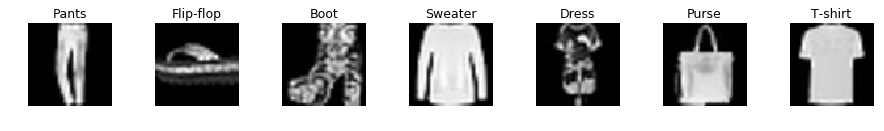
\includegraphics[width=\textwidth,height=2.5cm]{original_clothes}
			\caption{Samples of classes in clothes dataset. For easy understanding, we have labeled the classes with words}
			\label{fig:1}
		\end{center}
	\vskip -5mm
\end{figure*}

\begin{figure*}[tb]
	\vskip 5mm
		\begin{center}
			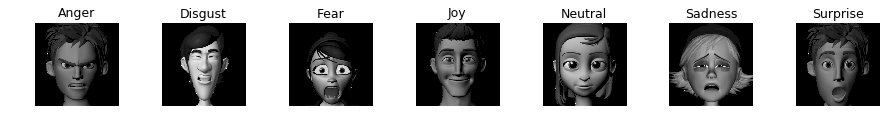
\includegraphics[width=\textwidth,height=2.5cm]{original_expressions}
			\caption{Samples of classes in expressions dataset. Each of the six characters is displayed}
			\label{fig:2}
		\end{center}
	\vskip -5mm
\end{figure*}

\subsection{Preprocessing}
\label{sec:preprocessing}
Both datasets are preprocessed in order to have comparable characteristics, as seen in Table (\ref{tab:1}). 

The clothes dataset is truncated to have seven classes, as there are only seven available classes within the expressions dataset. After converting every image to grayscale, both datasets are split into training and testing sets. This results in the clothes dataset having 42000 training examples and 7000 test samples, evenly distributed among seven classes; and the expressions dataset having 42000 training examples and 6300 testing samples.

Thereafter, every image contained within both datasets were resized to 64x64. This size allows for the maintenance of relevant features for facial expressions without increasing the computational resources in the training stage too much.

Finally, a series of transformations was performed in the test sets samples in order to increase the variability of the images. Rotation, blur, skew and shift transformations were randomly applied to each image as seen in Figures (\ref{fig:3}) and (\ref{fig:4}).

\begin{figure*}[!htb]
	\vskip 5mm
		\begin{center}
			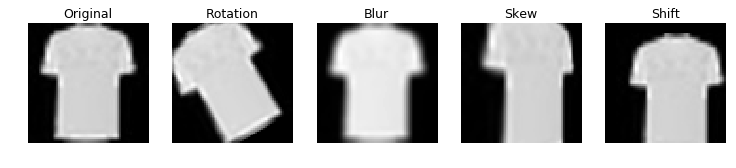
\includegraphics[height=2.5cm]{augmented_clothes}
			\caption{Transformations applied to samples in clothes test set}
			\label{fig:3}
		\end{center}
	\vskip -5mm
\end{figure*}

\begin{figure*}[!htb]
	\vskip 5mm
		\begin{center}
			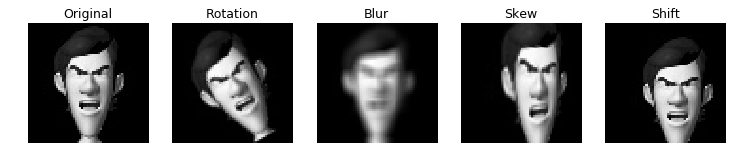
\includegraphics[height=2.5cm]{augmented_expressions}
			\caption{Transformations applied to samples in expressions test set}
			\label{fig:4}
		\end{center}
	\vskip -5mm
\end{figure*}

\subsection{Task and Evaluation}
\label{sec:evaluation}
The proposed task involves classification based on the labels provided by the datasets. Each experiment is evaluated based on the validation accuracy obtained in the last iteration of the training process. The results of the experiments are compared in two ways: comparison of the accuracy through different sizes of each dataset, and comparison of the accuracy between the same sizes of both datasets.

\section{Methodology}
\label{sec:methodology}
We examine the interim research questions (\ref{sec:irquestions}) to create a neural network architecture (\ref{sec:arch}). Based on our hypotheses, there are two main variables that we handle in every experiment: the dataset and its size. It follows that the rest of variables in the model such as any hyper-parameters, the activation functions, optimization strategies and others remain constant.

There are two categories of experiments to perform. In the first, one dataset is selected to train the model. The second category of experiment correspond to the size of the selected dataset. When performing these experiments, the same samples for the validation stage are used in order to make empirical comparisons of the accuracy. To do so, the test sets that were preprocessed earlier are utilised.


\subsection{Proposed Neural Network Architecture}
\label{sec:arch}

The proposed architecture is simple, containing one convolutional layer which is flattened and connected to a dense layer. The objective of this shallow structure is to have a model that extracts features at the same level in different datasets. It is important to take into consideration that the visually perceived differences in the clothes dataset are higher than in the expressions dataset. It follows that a deeper architecture might be able to extract more features from both datasets, but that information would be more relevant for expressions than for clothes.

Finally, relu and softmax activations along with max pooling layers are integrated into the structure of the network. Weights and biases of the convolutional layer are initialised with uniform distributions, whereas the parameters of the dense layer are initialised using the glorot strategy. The Adam learning rule is used to reduce the error of the system. The total number of training parameters within the network is 31637. 


\section{Baseline Experiments}
\label{sec:baseline}

The task outlined in section \ref{sec:evaluation} has been evaluated using the given datasets (\ref{sec:data}) in combination with the aforementioned methodology (\ref{sec:methodology}). The evaluation of this task provides a set of experimental results, as shown in table \label{tab:2} and \label{tab:3}. Both tables display the incremental reduction in dataset size and the classification accuracy of both employed datasets.

\begin{table*}[h]
  \centering
  \begin{tabular}{| l | l | l |}
    \hline
    \textbf{Size} & \textbf{Accuracy for clothes} & \textbf{Accuracy for expressions}\\ \hline
    100\% & 0.51 & 0.34\\ \hline
    75\% & 0.53  & 0.34\\ \hline
    50\% & 0.51 & 0.35\\ \hline
	25\% & 0.52 & 0.34\\ \hline
	10\% & 0.55 & 0.34\\ \hline
	1\% & 0.50 & 0.32\\ \hline
  \end{tabular}
  \caption{Validation accuracies for different sizes of the datasets}
  \label{tab:2}
\end{table*}
\begin{table*}[h]
  \centering
  \begin{tabular}{| l | l | l |}
    \hline
    \textbf{Size} & \textbf{Accuracy for clothes} & \textbf{Accuracy for expressions}\\ \hline
    100\% & 0.76 & 0.49\\ \hline
    75\% & 0.78  & 0.49\\ \hline
    50\% & 0.76 & 0.48\\ \hline
	25\% & 0.74 & 0.47\\ \hline
	10\% & 0.78 & 0.50\\ \hline
	1\% & 0.76 & 0.44\\ \hline
  \end{tabular}
  \caption{Validation accuracies for different sizes of the datasets using data augmentation}
  \label{tab:3}
\end{table*}
\section{Interim Conclusions}
\label{sec:conclusions}
The experimental results show that the first hypothesis stated in section \ref{sec:hypotheses} is proven to be true. To elaborate, a shallow network architecture may not be sufficient when classifying examples with subtle differences between classes. This is demonstrated within table \label{tab:2} and \label{tab:3}, where the classification accuracy for the clothes dataset is much greater than the accuracy for faces dataset \ref{sec:data}.

The classification accuracy presented within the results for both given datasets appears to remain fairly consistent regardless of the training set size. This suggests that the second hypothesis (H2) has been disproved. However, the hypothesis assumes that 1\% of the dataset is not enough data to sufficiently train the network.

\section{Future Work}
\label{sec:future}

To further investigate hypothesis two (H2), the dataset size could be reduced below 1\%. This future work would be motivated by \cite{cho2015much}, where it is shown that the classification accuracy is severely reduced when the size of the dataset falls below 100 training examples.

In the second phase of the project, two different transfer learning methods will be studied. These methods will serve as an investigation into the performance benefits of transfer learning given small datasets, which is a frequent occurrence in real world scenarios.

Firstly, a large pre-trained network (VGG16) \cite{DBLP:journals/corr/SimonyanZ14a} is transferred on our aforementioned baseline system (REF). The baseline system has pre-trained weights from a small dataset. The generality of this proposed model may be beneficial to train on images contained within the clothes dataset, since VGG16 trains on 200 types of common objects. In addition to transferring model parameters to domain-specific datasets, an investigation into transferring model parameters to datasets with unrelated and subtle differences between classes is presented. This is proposed in order to test the effectiveness of transfer learning on tasks that share little similarity with the tasks that the pre-trained (transferred) model was trained on.

Secondly, an investigation into the effectiveness of one-shot learning on small datasets is intended to be performed. To demonstrate a basic version of one-shot learning, an implementation of a Siamese network \cite{bromley1994signature} on either one of the two datasets will be executed. The principle of Siamese network is first to train a neural network to learn similarity measures by discriminating between a sets of same/different pairs of image \cite{koch2015}. The trained neural network is then implemented on one test image and all possible classes of images in pairwise manner , in an unseen dataset, and classification is done by finding the class with highest probability.   Our version of siamese network will be accomplished using existing models and additional modifications to these models, due to time constrains and the consideration of potential difficulty when implementing a one-shot learning architecture from scratch.

Finally, the proposed investigations would also aim to increase the accuracy of datasets with subtle difference between classes (such as the faces dataset). This would be conducted in an attempt to bring the classification accuracy of both proposed datasets into alignment.

\subsection{Backup Plans}
\label{sec:plans}

In instances where it is no longer possible to explore all proposed research avenues, a viable backup plan we intend to fall back to would be to solely concentrate on transfer learning(transferring pre-trained model or deep-feature extraction) but instead of the Siamese network for one-shot learning. 
\bibliographystyle{abbrv}
\bibliography{biblo.bib}

\end{document}
